\documentclass[11pt,a4paper]{article}
\usepackage[utf8]{inputenc}
\usepackage[T1]{fontenc}
\usepackage{lmodern}
\usepackage[margin=2.3cm]{geometry}
\usepackage{amsmath,amssymb}
\usepackage{booktabs,longtable,array}
\usepackage{graphicx}
\usepackage{fancyvrb}
\usepackage{xcolor}
\usepackage{forest}
\usepackage[hidelinks]{hyperref}

\renewcommand{\figurename}{Figura}
\renewcommand{\tablename}{Tabla}
\renewcommand{\contentsname}{Contenido}
\renewcommand{\refname}{Referencias}
\fvset{fontsize=\small,frame=single,framesep=2mm}
\newcommand{\eps}{\varepsilon}
\newcommand{\code}[1]{\texttt{#1}}

\title{Proyecto de Lenguajes Formales\\[2pt]
\large FIRST/FOLLOW, analizadores LL(1) y SLR(1), y evaluación de una SDD}
\author{Juan José Duque Marín \and Juan Lucas Ramírez Romero \and Samuel Pulgarin\\[4pt]
\small SI2002 Lenguajes Formales --- Universidad EAFIT}
\date{Noviembre de 2026}

\begin{document}
\maketitle
\tableofcontents

%======================================================================
\section{Introducción}
Este informe documenta la implementación, en Python~3 y usando solo la biblioteca estándar, de
los algoritmos de las secciones 4.4, 4.5, 4.6, 5.1 y 5.2 de Aho, Lam, Sethi y Ullman~\cite{aho}.
El programa calcula los conjuntos FIRST y FOLLOW (Ítem~1), decide si una gramática es LL(1) y/o
SLR(1) y analiza cadenas con el analizador correspondiente (Ítem~2), y evalúa una definición
dirigida por la sintaxis (SDD) sobre el árbol de análisis de una cadena mediante el grafo de
dependencias (Ítem~3). Las instrucciones de ejecución están en el \code{README.md}.

%======================================================================
\section{Algoritmos del libro y estructuras de datos}

\begin{longtable}{>{\raggedright}p{3.2cm} >{\raggedright}p{4.6cm} p{6.6cm}}
\toprule
\textbf{Parte} & \textbf{Libro} & \textbf{Implementación y estructuras de datos}\\
\midrule\endhead
Gramática & Convenciones del §2.2 del enunciado &
\code{grammar.py}. \code{Production} (dataclass inmutable: índice, cabeza, cuerpo como
\code{tuple[str]}; la producción-$\eps$ tiene cuerpo vacío). \code{Grammar}: lista de
producciones, \code{dict} cabeza $\to$ producciones, listas ordenadas de no terminales y
terminales.\\
FIRST & §4.4.2, reglas 1--3 de FIRST; FIRST de cadenas al final de §4.4.2 &
\code{first\_follow.py}. \code{dict[str, set[str]]}. Iteración de punto fijo: se recorren
todas las producciones hasta que ningún conjunto cambia. \code{first\_of\_string} implementa
FIRST$(X_1\cdots X_n)$; FIRST$(\eps)=\{\eps\}$.\\
FOLLOW & §4.4.2, reglas 1--3 de FOLLOW &
\code{dict[str, set[str]]}, punto fijo; \$ $\in$ FOLLOW$(S)$.\\
Prueba LL(1) & Definición al inicio de §4.4.3 (tres condiciones) &
\code{ll1.py}, \code{LL1.\_check\_condition}: para cada par de alternativas se verifican las
tres condiciones y se guarda una lista de violaciones legibles.\\
Tabla LL(1) & Algoritmo 4.31 &
\code{dict[(A, a), list[Production]]}; una celda con más de una producción es un conflicto.\\
Analizador LL(1) & Algoritmo 4.34, §4.4.4 &
Pila como \code{list} (tope al final) con \$ y $S$; devuelve la derivación por la izquierda (lista
de producciones emitidas) y, si se pide, la traza (Fig.~4.21).\\
Ítems LR(0) & §4.6.2 &
\code{slr.py}. \code{Item}: (producción, posición del punto), inmutable y \emph{hashable}.
Gramática aumentada con $S' \to S$; $S'$ se representa con la cadena \code{"S'"} (dos
caracteres) para que nunca choque con un no terminal de la entrada.\\
CLOSURE y GOTO & Fig.~4.32 y definición de GOTO en §4.6.2 &
CLOSURE recorre una lista que crece mientras se recorre (con un conjunto de ítems vistos).\\
Colección canónica & Fig.~4.33 &
Lista de estados (tuplas de ítems) + \code{dict[frozenset[Item], int]} para reconocer estados
repetidos + \code{dict[(i, X), j]} de transiciones. Los estados se numeran en orden BFS,
probando los símbolos en el orden en que aparecen tras el punto; así se reproduce la
numeración de la Fig.~4.31.\\
Tabla SLR(1) & Algoritmo 4.46, §4.6.4 &
ACTION: \code{dict[(i, a), list[Action]]} con acciones \code{("s", j)}, \code{("r", prod)},
\code{("acc", None)}; GOTO: \code{dict[(i, A), j]}. Los conflictos se guardan como
(estado, símbolo, acciones) y se clasifican en desplazamiento/reducción o reducción/reducción
(§4.5.4).\\
Analizador SLR(1) & Algoritmo 4.44, §4.6.3 &
Pila de estados (y una pila paralela de símbolos solo para la traza, Fig.~4.38). Devuelve la
secuencia de reducciones: la derivación por la derecha en orden inverso.\\
SDD como datos & §5.1.1, Fig.~5.1 &
\code{sdd/spec.py}. \code{AttrRef(pos, nombre)} (0 = cabeza, $1..k$ = cuerpo),
\code{Rule(target, deps, fn, texto)}, \code{SDD} (atributos sintetizados y heredados por
símbolo, reglas por producción, atributo principal). Las reglas se escriben con la notación del
libro ($R_1$, $N_2$\dots) y se traducen a posiciones.\\
Validación de la SDD & §5.1.1 y Step~2 del enunciado &
\code{validate}: cada regla define un sintetizado de la cabeza o un heredado de un no terminal del
cuerpo, usa solo atributos de su producción, cada atributo requerido se define exactamente una
vez y $S$ no tiene heredados.\\
Árbol de análisis & §5.1.2 &
\code{sdd/tree.py}. \code{Node}: id, símbolo, producción, hijos, \code{dict} de atributos. Un
solo \code{build\_tree} sirve para los dos analizadores: con LL(1) consume la derivación por la
izquierda en preorden; con SLR(1) invierte las reducciones (derivación por la derecha) y
construye los hijos de derecha a izquierda.\\
Grafo de dependencias & §5.2.1, Fig.~5.7 &
\code{sdd/depgraph.py}. Vértices: pares (id de nodo, atributo); aristas en listas de
adyacencia. Para cada nodo interior se instancian las reglas de \emph{su} producción, con una
arista desde cada atributo usado hacia el definido.\\
Orden de evaluación & §5.2.2 &
Algoritmo de Kahn con un \emph{heap} (desempate por (id, atributo), orden determinista). Si
quedan vértices sin procesar hay un ciclo; un DFS iterativo sobre esos vértices extrae un ciclo
concreto y se reporta \code{SDD is circular}.\\
Clasificación & §5.2.3 y §5.2.4 &
\code{classify}: comprobación automática de S-atribuida y L-atribuida, usada para contrastar la
justificación hecha a mano (§\ref{sec:clasif}).\\
\bottomrule
\end{longtable}

%======================================================================
\section{Ítems 1 y 2 con una gramática propia}
Usamos una gramática de listas anidadas, como \code{(i,(i,i),())}, que no aparece en el
enunciado:
\begin{Verbatim}
4
S -> (A)
A -> BC e
C -> ,BC e
B -> i S
\end{Verbatim}
Tiene producciones-$\eps$, recursión indirecta ($S \Rightarrow (A) \Rightarrow (BC) \Rightarrow
(SC)$) y FOLLOW que exige varias iteraciones. Todo lo siguiente fue calculado por el programa
(\code{python3 main.py --sets --verbose --trace < examples/report\_grammar.txt}).

\subsection{FIRST y FOLLOW}
\begin{Verbatim}
First(A) = {(, i, e}
First(B) = {(, i}
First(C) = {,, e}
First(S) = {(}
Follow(A) = {)}
Follow(B) = {), ,}
Follow(C) = {)}
Follow(S) = {), ,, $}
\end{Verbatim}

\subsection{Tabla LL(1)}
Las tres condiciones de §4.4.3 se cumplen; por ejemplo, para $A \to BC \mid \eps$:
FIRST$(BC)=\{(,i\}$ y FOLLOW$(A)=\{)\}$ son disjuntos. La tabla (Algoritmo~4.31) no tiene
entradas múltiples:
\begin{Verbatim}
   (         )       ,         i        $
-  --------  ------  --------  -------  -
A  A -> BC   A -> e            A -> BC
B  B -> S                      B -> i
C            C -> e  C -> ,BC
S  S -> (A)
\end{Verbatim}

\subsection{Autómata LR(0) y tabla SLR(1)}
La Figura~\ref{fig:lr0} muestra la colección canónica (Fig.~4.33) dibujada por nuestro
visualizador; la tabla SLR(1) (Algoritmo~4.46) no tiene conflictos, así que la gramática es
LL(1) y SLR(1).
\begin{figure}[h]
\centering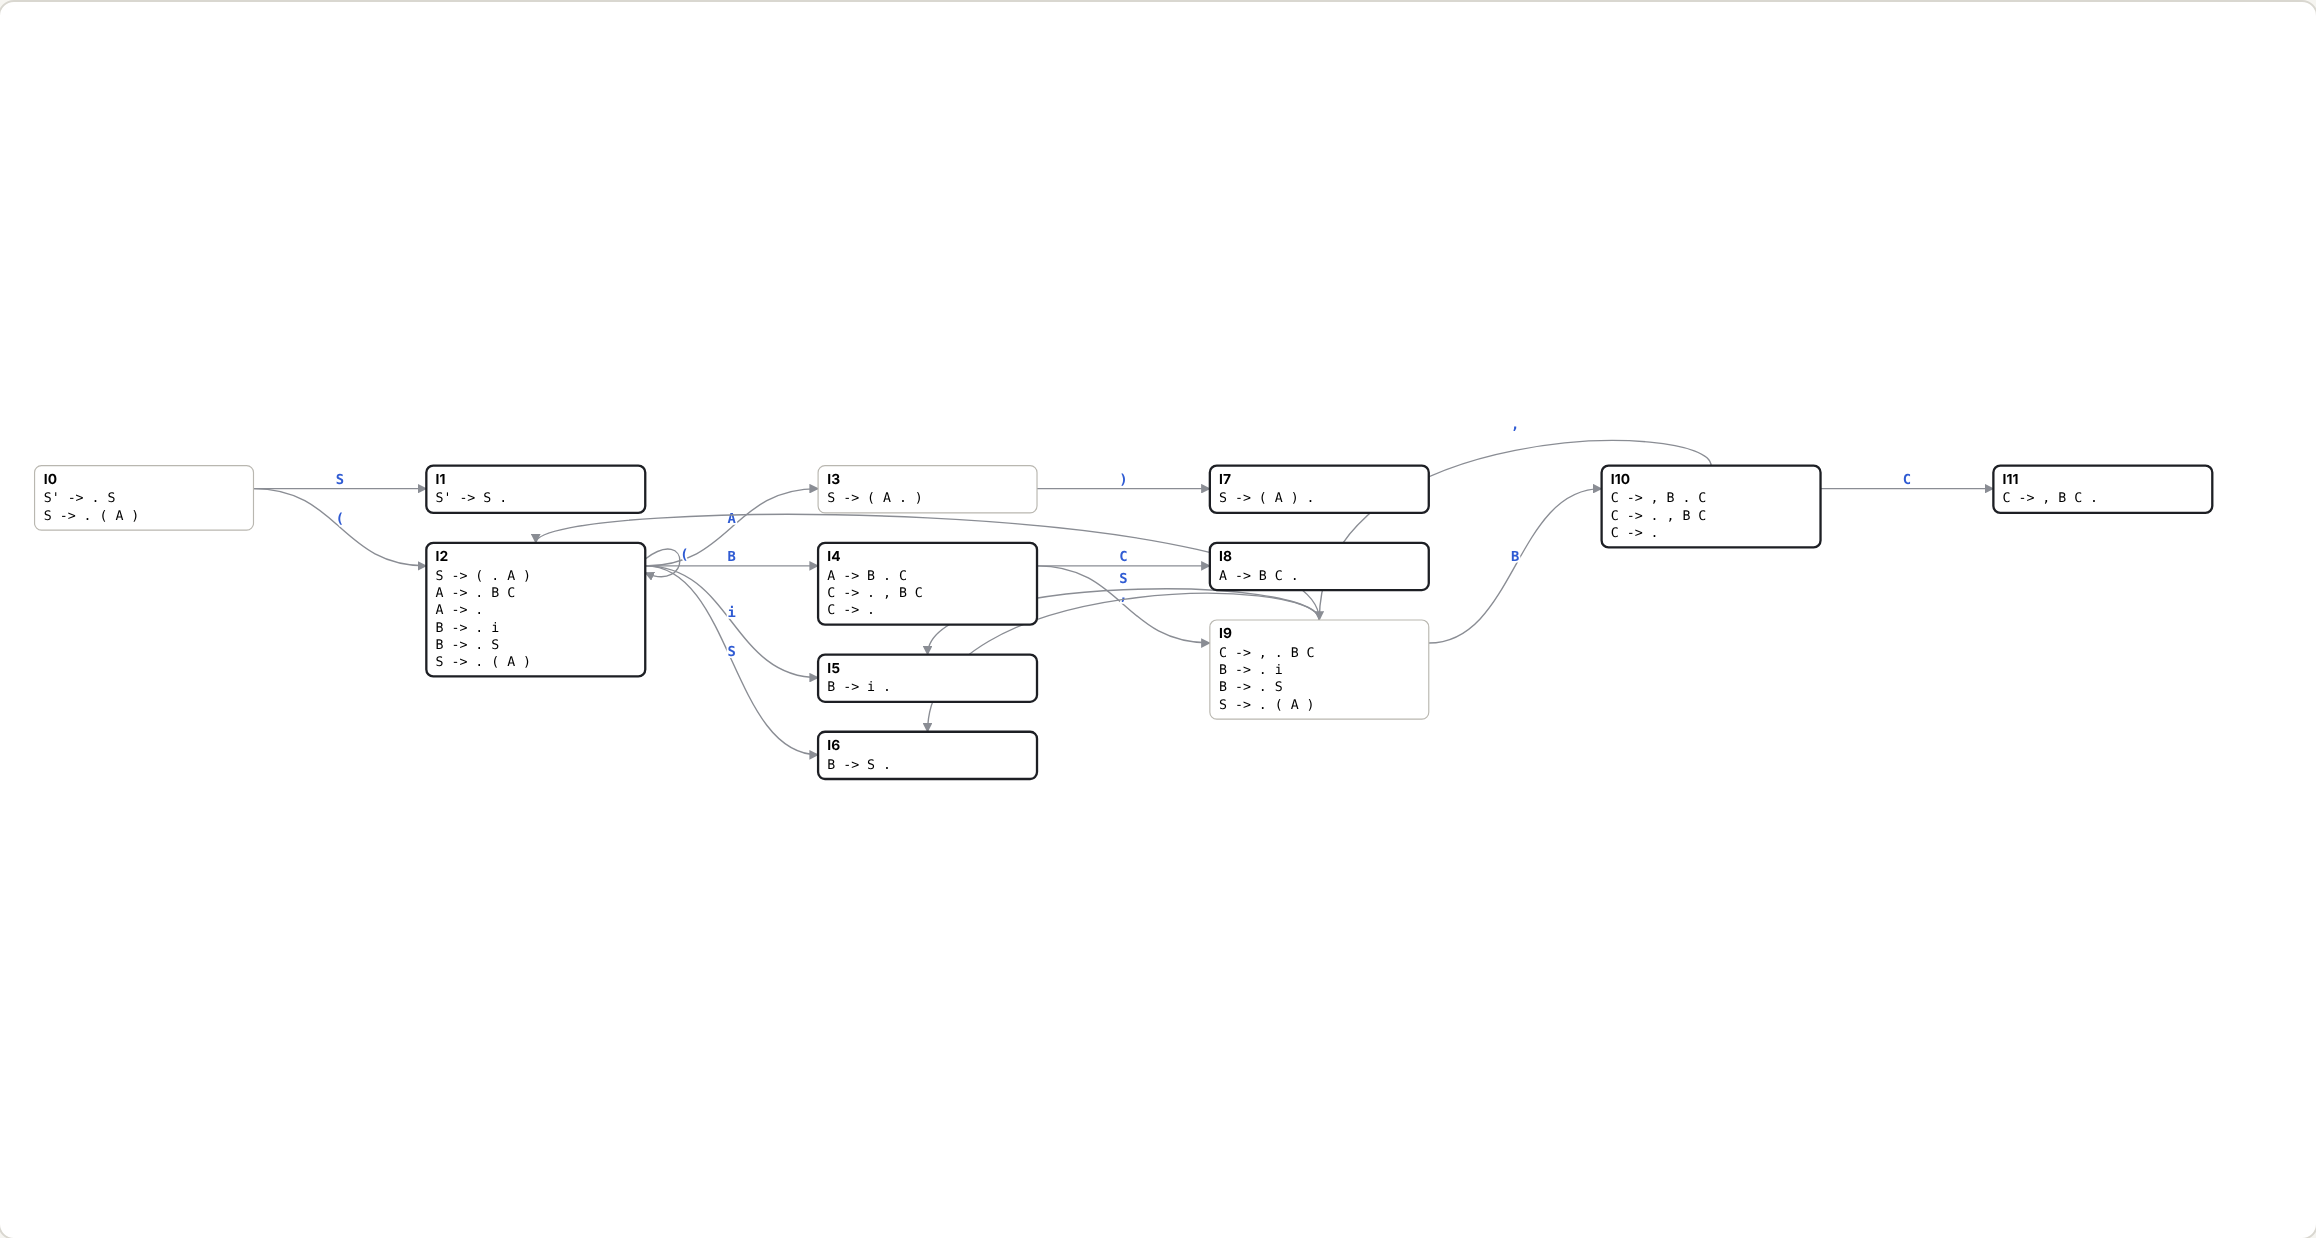
\includegraphics[width=\linewidth]{fig_lr0.png}
\caption{Autómata LR(0) de la gramática de listas anidadas.}\label{fig:lr0}
\end{figure}

\begin{Verbatim}
state  (   )            ,            i   $            A  B   C   S
-----  --  -----------  -----------  --  -----------  -  --  --  -
0      s2                                                        1
1                                        acc
2      s2  r(A -> e)                 s5               3  4       6
3          s7
4          r(C -> e)    s9                                   8
5          r(B -> i)    r(B -> i)
6          r(B -> S)    r(B -> S)
7          r(S -> (A))  r(S -> (A))      r(S -> (A))
8          r(A -> BC)
9      s2                            s5                  10      6
10         r(C -> e)    s9                                   11
11         r(C -> ,BC)
\end{Verbatim}

\subsection{Una cadena analizada paso a paso}
Cadena \code{(i,())} con el analizador LL(1) (Algoritmo~4.34; formato de la Fig.~4.21):
\begin{Verbatim}
MATCHED  STACK        INPUT    ACTION
         S $          (i,())$  output S -> (A)
         ( A ) $      (i,())$  match (
(        A ) $        i,())$   output A -> BC
(        B C ) $      i,())$   output B -> i
(        i C ) $      i,())$   match i
(i       C ) $        ,())$    output C -> ,BC
(i       , B C ) $    ,())$    match ,
(i,      B C ) $      ())$     output B -> S
(i,      S C ) $      ())$     output S -> (A)
(i,      ( A ) C ) $  ())$     match (
(i,(     A ) C ) $    ))$      output A -> e
(i,(     ) C ) $      ))$      match )
(i,()    C ) $        )$       output C -> e
(i,()    ) $          )$       match )
(i,())   $            $        accept
\end{Verbatim}
La misma cadena con el analizador SLR(1) (Algoritmo~4.44; formato de la Fig.~4.38):
\begin{Verbatim}
STACK          SYMBOLS  INPUT    ACTION
0                       (i,())$  shift 2
0 2            (        i,())$   shift 5
0 2 5          (i       ,())$    reduce by B -> i
0 2 4          (B       ,())$    shift 9
0 2 4 9        (B,      ())$     shift 2
0 2 4 9 2      (B,(     ))$      reduce by A -> e
0 2 4 9 2 3    (B,(A    ))$      shift 7
0 2 4 9 2 3 7  (B,(A)   )$       reduce by S -> (A)
0 2 4 9 6      (B,S     )$       reduce by B -> S
0 2 4 9 10     (B,B     )$       reduce by C -> e
0 2 4 9 10 11  (B,BC    )$       reduce by C -> ,BC
0 2 4 8        (BC      )$       reduce by A -> BC
0 2 3          (A       )$       shift 7
0 2 3 7        (A)      $        reduce by S -> (A)
0 1            S        $        accept
\end{Verbatim}

%======================================================================
\section{Ítem 3: definición dirigida por la sintaxis}

\subsection{Gramática}
La SDD calcula el valor de un número escrito en una base arbitraria. La cadena $b{:}d_1\cdots
d_k$ significa ``los dígitos $d_1\cdots d_k$ leídos en base $b$'', donde la base $b$ se escribe
en decimal: \code{8:17} vale $1\cdot 8+7=15$ y \code{12:11} vale $13$.
\begin{Verbatim}
4
S -> N:N
N -> DR
R -> DR e
D -> 0 1 2 3 4 5 6 7 8 9
\end{Verbatim}
Cumple G1 (convenciones del §2.2; es LL(1) y SLR(1): FIRST$(DR)$ son los dígitos y
FOLLOW$(R)=\{:,\$\}$), G2 (4 no terminales, 14 producciones, $R$ es recursivo) y G3: no es
ninguna de las SDD del libro ni del enunciado. A diferencia de las SDD de la Fig.~5.4 (expresiones)
o de los números binarios, aquí el valor de un subárbol (la base, $N_1.val$) se convierte en
atributo heredado del subárbol hermano ($N_2.base$), y el valor se acumula de izquierda a derecha
con la regla de Horner mediante un heredado ($R.acc$).

\subsection{Tabla de atributos}
\begin{tabular}{llllp{6.4cm}}
\toprule
\textbf{Símbolo} & \textbf{Atributo} & \textbf{Clase} & \textbf{Tipo} & \textbf{Significado}\\
\midrule
$S$ & $val$ & sintetizado & entero / error & valor del número (atributo principal); error si algún
dígito no es menor que su base\\
$S$ & $ok$ & sintetizado & booleano & los dos números están bien formados\\
$N$ & $base$ & heredado & entero & base en la que se leen los dígitos de $N$\\
$N$ & $val$ & sintetizado & entero & valor del número\\
$N$ & $ok$ & sintetizado & booleano & todos los dígitos de $N$ son menores que la base\\
$R$ & $base$ & heredado & entero & la misma base, pasada a lo largo de la lista\\
$R$ & $acc$ & heredado & entero & valor de los dígitos a la izquierda de $R$ (Horner)\\
$R$ & $val$ & sintetizado & entero & valor de toda la lista de dígitos\\
$R$ & $ok$ & sintetizado & booleano & todos los dígitos de la lista son menores que la base\\
$D$ & $v$ & sintetizado & entero & valor numérico del dígito\\
dígitos y \code{:} & $lexval$ & sintetizado & carácter & el propio carácter (lo da el
``escáner'')\\
\bottomrule
\end{tabular}

\subsection{Reglas semánticas}
En el formato de la Fig.~5.1 (los símbolos repetidos llevan subíndice):

\begin{tabular}{ll}
\toprule
\textbf{Producción} & \textbf{Reglas semánticas}\\
\midrule
$S \to N_1 : N_2$ & $N_1.base = 10$\\
 & $N_2.base = N_1.val$\\
 & $S.val = N_2.val$ si $N_1.ok \wedge N_2.ok$, si no \emph{error}\\
 & $S.ok = N_1.ok \wedge N_2.ok$\\
\midrule
$N \to D\,R$ & $R.base = N.base$\\
 & $R.acc = D.v$\\
 & $N.val = R.val$\\
 & $N.ok = (D.v < N.base) \wedge R.ok$\\
\midrule
$R \to D\,R_1$ & $R_1.base = R.base$\\
 & $R_1.acc = R.acc \cdot R.base + D.v$\\
 & $R.val = R_1.val$\\
 & $R.ok = (D.v < R.base) \wedge R_1.ok$\\
\midrule
$R \to \eps$ & $R.val = R.acc$\\
 & $R.ok = \mathit{true}$\\
\midrule
$D \to d$ \quad ($d \in \{0,\dots,9\}$) & $D.v = \mathrm{int}(d.lexval)$\\
\bottomrule
\end{tabular}

\medskip
Comprobación de §5.1.1: en cada producción, cada sintetizado de la cabeza y cada heredado de un
no terminal del cuerpo se define exactamente una vez (por ejemplo, en $R \to DR_1$ se definen
$R.val$, $R.ok$, $R_1.base$ y $R_1.acc$); ninguna regla usa atributos de símbolos fuera de su
producción; $S$ no tiene heredados. El validador estático del programa verifica lo mismo.

\subsection{Ejemplo resuelto: la cadena \code{2:101}}
La cadena tiene 5 terminales y vale $1\cdot 4 + 0\cdot 2 + 1 = 5$. La Figura~\ref{fig:tree}
es el árbol anotado; los números \#$k$ son los identificadores de los nodos en preorden, que
usamos para nombrar los vértices del grafo.

\begin{figure}[h]
\centering\small
\begin{forest}
for tree={font=\small, s sep=4mm, l sep=6mm, align=center}
[{$S$\#0\\ $val=5$, $ok$}
  [{$N$\#1\\ $base=10$\\ $val=2$, $ok$}
    [{$D$\#2\\ $v=2$} [{\code{2}\#3}]]
    [{$R$\#4\\ $base=10$, $acc=2$\\ $val=2$, $ok$} [{$\eps$\#5}]]]
  [{\code{:}\#6}]
  [{$N$\#7\\ $base=2$\\ $val=5$, $ok$}
    [{$D$\#8\\ $v=1$} [{\code{1}\#9}]]
    [{$R$\#10\\ $base=2$, $acc=1$\\ $val=5$, $ok$}
      [{$D$\#11\\ $v=0$} [{\code{0}\#12}]]
      [{$R$\#13\\ $base=2$, $acc=2$\\ $val=5$, $ok$}
        [{$D$\#14\\ $v=1$} [{\code{1}\#15}]]
        [{$R$\#16\\ $base=2$, $acc=5$\\ $val=5$, $ok$} [{$\eps$\#17}]]]]]]
\end{forest}
\caption{Árbol de análisis anotado de \code{2:101} ($ok$ = $\mathit{true}$ en todos los nodos).}
\label{fig:tree}
\end{figure}

La Figura~\ref{fig:dep} es el grafo de dependencias (§5.2.1): un vértice por cada atributo de
cada nodo (los heredados a la izquierda del nodo y los sintetizados a la derecha, como en la
Fig.~5.7) y una arista desde cada atributo usado hacia el atributo definido. Lo más
interesante es la arista $N\#1.val \to N\#7.base$, que lleva información de un subárbol a su
hermano derecho, y la cadena $R\#10.acc \to R\#13.acc \to R\#16.acc \to R\#16.val \to R\#13.val
\to R\#10.val \to N\#7.val \to S\#0.val$, que baja por la lista acumulando el valor y luego lo
sube.

\begin{figure}[h]
\centering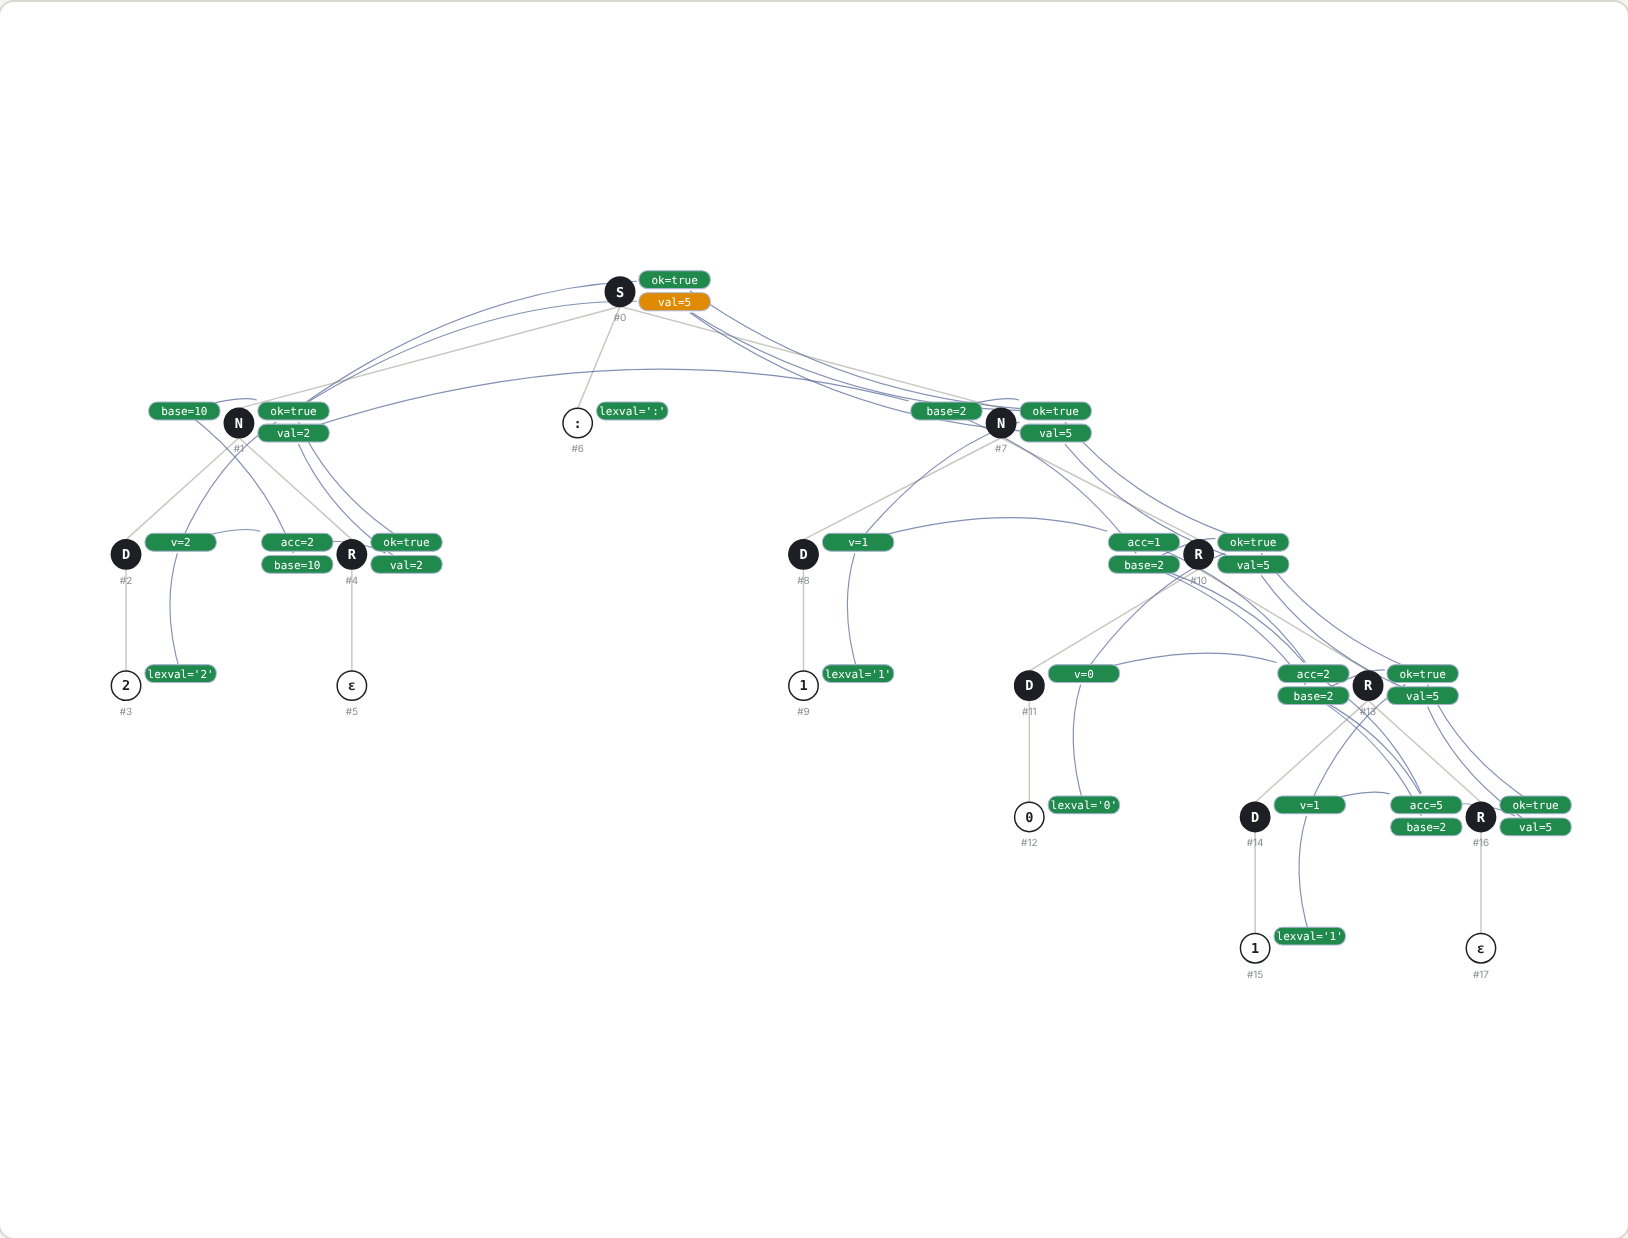
\includegraphics[width=\linewidth]{fig_depgraph.png}
\caption{Grafo de dependencias de \code{2:101}, con todos los atributos evaluados (visualizador).}
\label{fig:dep}
\end{figure}

Un orden de evaluación válido es el orden topológico que produce el programa
(\code{python3 main.py --sdd < examples/sdd\_hand.txt}):
\begin{Verbatim}[fontsize=\footnotesize]
 1. N#1.base = 10       12. 1#9.lexval = '1'    23. R#16.base = 2
 2. 2#3.lexval = '2'    13. D#8.v = 1           24. R#16.ok = True
 3. D#2.v = 2           14. R#10.acc = 1        25. R#13.ok = True
 4. R#4.acc = 2         15. R#10.base = 2       26. R#10.ok = True
 5. R#4.base = 10       16. 0#12.lexval = '0'   27. N#7.ok = True
 6. R#4.ok = True       17. D#11.v = 0          28. S#0.ok = True
 7. N#1.ok = True       18. R#13.acc = 2        29. R#16.val = 5
 8. R#4.val = 2         19. R#13.base = 2       30. R#13.val = 5
 9. N#1.val = 2         20. 1#15.lexval = '1'   31. R#10.val = 5
10. :#6.lexval = ':'    21. D#14.v = 1          32. N#7.val = 5
11. N#7.base = 2        22. R#16.acc = 5        33. S#0.val = 5
\end{Verbatim}
Cada vértice aparece después de todos sus predecesores; por ejemplo $N\#7.base$ (paso 11) va
después de $N\#1.val$ (paso 9), y $R\#16.acc = R\#13.acc\cdot R\#13.base + D\#14.v = 2\cdot 2+1
= 5$ (paso 22) va después de los pasos 18, 19 y 21.

\subsection{Clasificación}\label{sec:clasif}
\textbf{No es S-atribuida}: según §5.2.3, una SDD es S-atribuida si todos sus atributos son
sintetizados, y la nuestra tiene heredados ($N.base$, $R.base$, $R.acc$). De hecho, como el
enunciado exige al menos un heredado, ninguna SDD válida del proyecto puede ser S-atribuida.

\textbf{Sí es L-atribuida} (§5.2.4): todo atributo es sintetizado, o es heredado y su regla en
$A \to X_1\cdots X_n$ que define $X_i.a$ usa solo (a) heredados de la cabeza $A$, (b) atributos
de $X_1,\dots,X_{i-1}$ o (c) atributos de $X_i$ sin formar ciclos. Revisamos cada heredado:
\begin{itemize}
\item $S \to N_1 : N_2$: $N_1.base = 10$ no usa nada; $N_2.base = N_1.val$ usa un atributo de
$N_1$, que está a la izquierda de $N_2$ (b).
\item $N \to DR$: $R.base = N.base$ usa un heredado de la cabeza (a); $R.acc = D.v$ usa $D$, a la
izquierda de $R$ (b).
\item $R \to DR_1$: $R_1.base = R.base$ (a); $R_1.acc = R.acc\cdot R.base + D.v$ usa heredados de
la cabeza (a) y $D$, a la izquierda de $R_1$ (b).
\end{itemize}
Las demás reglas definen atributos sintetizados. La función \code{classify} del programa da el
mismo resultado (\code{S-attributed: no, L-attributed: yes}). Aunque sea L-atribuida, el
evaluador usa el método general del grafo de dependencias (Step~5).

\subsection{Pruebas}\label{sec:pruebas}
Salida de \code{python3 main.py --sdd < examples/sdd\_tests.txt} (se muestra solo el
resultado; el programa también imprime el árbol y el orden para cada cadena):

\begin{tabular}{lll}
\toprule
\textbf{Cadena} & \textbf{Por qué} & \textbf{Resultado}\\
\midrule
\code{2:0} & la más corta del lenguaje (3 terminales) & $S.val = 0$\\
\code{8:17} & caso típico & $S.val = 15$\\
\code{12:11} & base de dos dígitos (usa $N_2.base = N_1.val$) & $S.val = 13$\\
\code{9:9} & dígito no menor que la base & $S.val = $ \emph{error}, $S.ok = \mathit{false}$\\
\code{8:1x} & no está en el lenguaje & \code{no}\\
\code{2:1}$^{40}$ & recursión profunda (40 nodos $R$ anidados) & $S.val = 2^{40}-1 = 1099511627775$\\
\bottomrule
\end{tabular}

\medskip
Las pruebas automáticas (\code{tests/test\_sdd.py}) verifican además que las cadenas den el
mismo árbol y el mismo valor con los dos analizadores, que el orden producido es realmente
topológico (cada arista va de un vértice anterior a uno posterior) y una cadena con 60 dígitos.

\subsection{Experimento de circularidad}
En \code{sdd/my\_sdd\_circular.py} cambiamos una sola regla:
\[
N \to DR:\qquad R.acc = D.v \quad\leadsto\quad R.acc = R.val + D.v .
\]
La SDD sigue siendo sintácticamente válida (el validador la acepta: $R.acc$ sigue siendo un
heredado de un símbolo del cuerpo, definido una vez), pero ahora $R.acc$ depende de $R.val$, y
$R.val$ depende ---bajando por la lista hasta $R \to \eps$, donde $R.val = R.acc$--- de $R.acc$.
La clasificación automática ya la marca como no L-atribuida, y el evaluador detecta el ciclo en
el grafo de cada árbol:
\begin{Verbatim}[fontsize=\footnotesize]
$ python3 main.py --sdd --circular < examples/sdd_hand.txt
SDD: number in an arbitrary base (circular)
Parser: LL(1)
S-attributed: no   L-attributed: no
  (not S-attributed: there are inherited attributes)
  (not L-attributed: in N -> DR, R.acc uses R.val, a synthesized attribute of the same
   symbol (may be circular))

String: 2:101
SDD is circular: R#16.acc -> R#16.val -> R#13.val -> R#10.val -> R#10.acc -> R#13.acc
                 -> R#16.acc
\end{Verbatim}
\begin{figure}[h]
\centering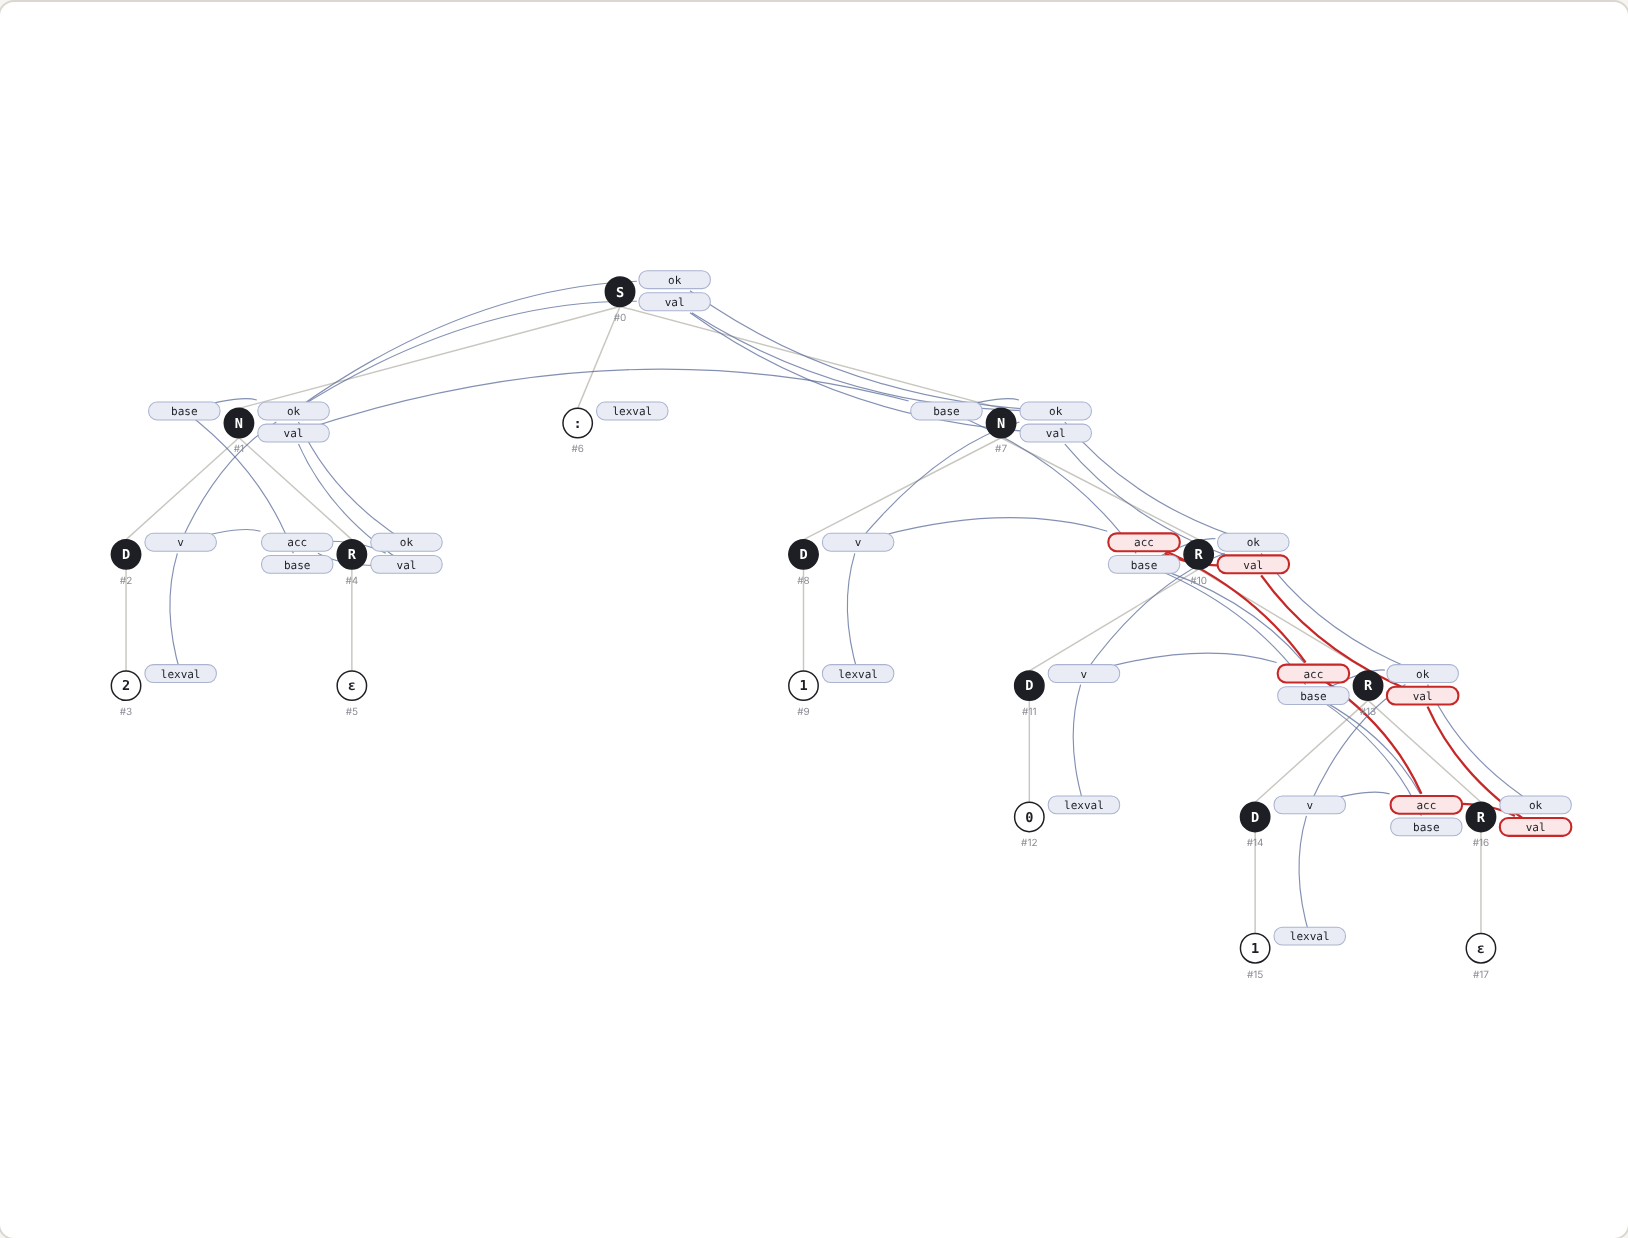
\includegraphics[width=\linewidth]{fig_circular.png}
\caption{Grafo de dependencias de \code{2:101} con la SDD mutada; el ciclo está en rojo.}
\end{figure}

%======================================================================
\section{Pruebas de los Ítems 1 y 2}
\code{tests/test\_parsers.py} (ejecutar con \code{python3 -m unittest discover -s tests}) compara
con resultados del libro y del enunciado:
\begin{itemize}
\item FIRST y FOLLOW de la gramática (4.28) (Ejemplo~4.30), la tabla de la Fig.~4.17 y los
movimientos de la Fig.~4.21.
\item El autómata LR(0) de la Fig.~4.31 (12 estados con la misma numeración), la tabla SLR de la
Fig.~4.37 (36 entradas ACTION y la tabla GOTO completa) y los 14 movimientos de la Fig.~4.38.
\item La salida exacta de los Ejemplos 1, 2 y 3 del enunciado y los cuatro casos de
clasificación; para ``LL(1) pero no SLR(1)'' usamos $S \to AaAb \mid BbBa$, $A \to \eps$,
$B \to \eps$, que tiene conflictos reducción/reducción en el estado 0.
\item Casos borde: $S \to \eps$, la cadena \code{e}, símbolos que no están en la gramática (incluido
\code{\$}), alternativas duplicadas, la primera línea no es la de $S$, finales de línea de
Windows, fin de archivo sin línea vacía y un FOLLOW que necesita varias pasadas.
\end{itemize}
Las 36 pruebas pasan con Python 3.11 y 3.13.

%======================================================================
\section{Problemas encontrados y cómo los resolvimos}
\begin{enumerate}
\item \textbf{Orden de impresión de los conjuntos.} El enunciado pide los terminales en orden
ASCII, luego \code{e} y luego \code{\$}. Como \code{\$} (ASCII 36) es menor que las letras y los
dígitos, un \code{sorted} directo lo ponía primero. Se ordenan solo los terminales y se agregan
\code{e} y \code{\$} al final. Queda una ambigüedad: si se imprimen todas las líneas
\code{First} y luego todas las \code{Follow}, o intercaladas por no terminal; lo dejamos en una
constante (\code{SETS\_GROUPED}) para cambiarlo según lo que diga el profesor.
\item \textbf{Condición LL(1) frente a conflictos en la tabla.} Implementamos la definición de
§4.4.3 y además verificamos que la tabla no tenga entradas múltiples. Pensábamos que las dos
pruebas siempre coinciden, pero no es así cuando un no terminal es inalcanzable desde $S$: si
tiene dos alternativas que derivan $\eps$, FOLLOW es vacío, la condición~2 falla y la tabla no
tiene conflicto. Exigimos las dos.
\item \textbf{El símbolo $S'$.} Como los símbolos de la entrada son de un carácter, cualquier
letra que usáramos para el nuevo símbolo inicial podía chocar con uno real. Usamos la cadena
\code{"S'"}, que no puede aparecer en la entrada.
\item \textbf{Numeración de estados.} Para comparar con la Fig.~4.31 y con nuestros cálculos a
mano, el orden de los estados tenía que ser predecible. Recorremos los estados en BFS y, dentro
de cada uno, los símbolos en el orden en que aparecen después del punto.
\item \textbf{Árbol desde el analizador SLR(1).} El algoritmo~4.44 no construye el árbol. Primero
pensamos usar una pila de nodos durante el análisis, pero preferimos que ambos analizadores
devuelvan su derivación: invertir las reducciones da la derivación por la derecha, y basta
expandir los hijos de derecha a izquierda (consumiendo la entrada desde el final). Una prueba
verifica que los dos analizadores producen el mismo árbol.
\item \textbf{Símbolos repetidos en una producción.} En $S \to N:N$ hay que distinguir
$N_1$ de $N_2$. Las reglas se escriben con los subíndices del libro y una función los traduce a
posiciones del cuerpo.
\item \textbf{Hojas $\eps$.} El nodo $\eps$ es un hijo en el árbol pero no un símbolo del cuerpo
de la producción; al instanciar las reglas se omite para que las posiciones coincidan.
\item \textbf{Clasificación de la SDD mutada.} La primera versión de \code{classify} aceptaba que
un heredado de $X_i$ usara cualquier atributo de $X_i$ (condición (c) de §5.2.4) y por eso
declaraba L-atribuida la SDD circular. La condición (c) exige que no haya ciclos; como un
sintetizado de $X_i$ puede depender de sus heredados, ahora solo aceptamos otros heredados de
$X_i$.
\item \textbf{Valor de una cadena con dígitos inválidos.} Con \code{9:9} el valor principal
salía 9 aunque el número estuviera mal formado. Hicimos que $S.val$ dependa también de $N_1.ok$
y $N_2.ok$.
\item \textbf{Un valor esperado mal contado en las pruebas.} Habíamos escrito que la Fig.~4.37
tiene 41 entradas ACTION; al contar de nuevo fila por fila son 36, que es lo que da el programa.
\end{enumerate}

\begin{thebibliography}{9}
\bibitem{aho} A.~V. Aho, M.~S. Lam, R.~Sethi y J.~D. Ullman. \emph{Compilers: Principles,
Techniques, and Tools}, 2.ª ed. Addison-Wesley, 2006.
\end{thebibliography}
\end{document}
